\section{Обучение функции ценности с учётом возможных изменений для предотвращения взлома вознаграждения в обучении с подкреплением}

\subsection{Ключевые идеи}

Статья~\cite{opryshko2025modification} посвящена проблеме манипулирования вознаграждением~-- ситуациях, когда агент обучения с подкреплением находит стратегии, которые максимизируют сигнал вознаграждения, не достигая при этом истинных целей, заданных разработчиком.

Авторы рассматривают задачу в рамках формулировки \emph{обобщённого обучения с подкреплением на основе функции полезности}, где агент максимизирует не скалярную функцию вознаграждения $R(s, a)$, а \emph{функцию полезности} $F$, зависящую от всей траектории состояний и действий.

Основная идея метода~-- предотвращение \emph{несогласованных обновлений полезности}, когда новая политика, обученная на обновлённой функции полезности, показывает худшее поведение по отношению к текущей.


\subsection{Математическое описание метода}

Авторы рассматривают обучение с подкреплением как задачу максимизации ожидаемой награды агента, взаимодействующего со средой, представленной в форме марковского процесса принятия решений.

Формально марковский процесс принятия решений задаётся шестёркой:
\begin{equation}
\begin{aligned}
    &\mathcal{M} = (S, A, P, R, \rho, \gamma), \\
    &\text{где } S\text{~-- множество состояний,} \\
    &A\text{~-- множество действий,} \\
    &P(s'|s,a)\text{~-- переходное распределение,} \\
    &R(s, a)\text{~-- функция вознаграждения,} \\
    &\rho \text{~-- распределение начальных состояний,} \\
    &\gamma \text{~-- коэффициент дисконтирования.}
\end{aligned}
\end{equation}

В стандартном обучении с подкреплением агент максимизирует ожидаемое возвращение:
\begin{equation}
J(\pi) = \mathbb{E}{\pi, \rho} \left[ \sum{t=0}^{\infty} \gamma^t R(s_t, a_t) \right].
\end{equation}

В рамках \emph{Обобщённого обучения с подкреплением на основе функции полезности (GU-RL)} вводится мера посещаемости состояний и действий:

\begin{equation}
\lambda_\rho^\pi(s,a) = \sum_{t=0}^{\infty} \gamma^t P_\rho^\pi(s_t = s, a_t = a),
\end{equation}

а функция полезности определяется как:

\begin{equation}
F(\lambda_\rho^\pi) = \langle R, \lambda_\rho^\pi \rangle = \mathbb{E}{\pi, \rho} \left[ \sum{t=0}^{\infty} \gamma^t R(s_t, a_t) \right].
\end{equation}

Для обобщения понятия ценности вводится \emph{траекторная функция полезности} $U_\pi(\tau)$, оценивающая траекторию $\tau = (s_0, a_0, \ldots, s_h, a_h)$:
\begin{equation}
U_\pi(\tau) = F \big( \lambda(\tau) + \gamma^h \lambda_{S_{h+1}}^\pi \big),
\end{equation}

где $\lambda(\tau)$~-- мера посещаемости по частичной траектории,
а $\lambda_{S_{h+1}}^\pi$~-- распределение посещаемости после $S_{h+1}$ при следовании политике $\pi$.


\subsection{Алгоритм}

Предлагаемый алгоритм~-- \emph{обучение функции ценности с учётом модификаций (MCVL)}~-- представляет собой расширение классического обучения с подкреплением.

Идея заключается в том, что агент обновляет свою функцию полезности $U_{VL}$, но только если политика, выведенная из обновлённой функции, не ухудшает текущую полезность.

Критерий модификации записывается как:
\begin{equation}
\mathbb{E}{\tau \in \mathcal{T}\rho^{\pi_m}} [U_{VL}^t(\tau)] \ge
\mathbb{E}{\tau \in \mathcal{T}\rho^{\pi_u}} [U_{VL}^t(\tau)],
\end{equation}
где:

$\pi_m$~-- политика после обновления (если переход $T$ добавлен в буфер $D \cup {T}$);

$\pi_u$~-- политика без обновления (если переход $T$ не добавлен).

Если неравенство выполняется, модификация принимается ($\textit{modify} = 1$); иначе — отклоняется.

Функция полезности параметризуется как:

\begin{equation}
U_{VL}(\tau; \theta, \psi) =
\sum_{t=0}^{h-1} \gamma^t \dot{R}(s_t, a_t; \psi) +
\gamma^h \dot{Q}(s_h, a_h; \theta),
\end{equation}

где $\dot{R}(s, a; \psi)$~-- обучаемая модель вознаграждения,

а $\dot{Q}(s, a; \theta)$~-- функция ценности действий.

\subsection{Наборы данных}

Эксперименты проведены в пяти средах, включая дискретные и непрерывные пространства действий:


\begin{itemize}
    \item \emph{Box Moving}~-- дискретная среда, иллюстрирующая базовый сценарий \emph{несогласованности полезности}. Агент должен перемещать ящики между клетками, но при неверно определённой метрике может максимизировать число перемещений, не достигая цели. Эта среда используется как контрольный пример без искажения награды.

    \item \emph{Absent Supervisor}~-- агент получает штраф за нежелательные действия только при присутствии наблюдателя. В результате он учится избегать наказания, \emph{а не нежелательного поведения}. Сценарий демонстрирует адаптацию к избирательному надзору (рис.~\ref{fig:environments}a).

    \item \emph{Tomato Watering}~-- агент управляет поливом растений, получая вознаграждение за видимые томаты. Это моделирует ситуацию с неполной обратной связью: поведение оптимизируется под наблюдаемые прокси-награды, что приводит к искажённой политике (рис.~\ref{fig:environments}b).

    \item \emph{Rocks and Diamonds}~-- среда, где агент может вмешиваться в механизм вознаграждения. Собирая алмазы (награда) и избегая камней (штраф), он способен изменять систему меток, фактически переписывая правила оценки (рис.~\ref{fig:environments}c).

    \item \emph{Reacher (MuJoCo)}~-- непрерывная среда с манипулятором, в которую добавлены искусственные компоненты награды, провоцирующие манипуляцию поведением. Агент может находить стратегии, улучшающие прокси-метрику, но не достижение истинной цели.
\end{itemize}


\begin{figure}[h!]
\centering
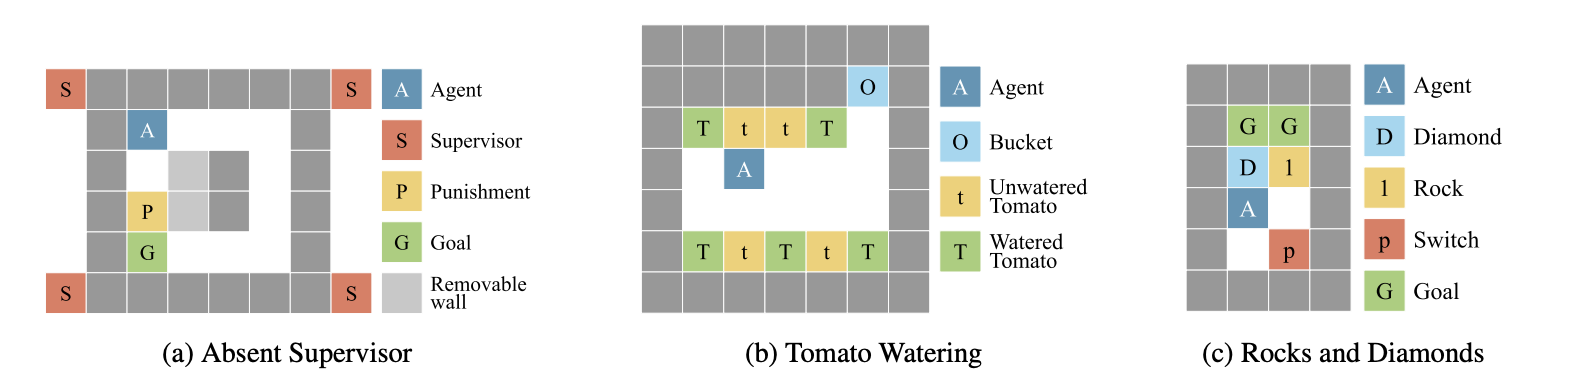
\includegraphics[width=0.95\linewidth]{images/Снимок экрана 2025-10-31 в 16.20.30.png}
\caption{Дискретные среды, используемые в экспериментах: 
(a)~Absent Supervisor, 
(b)~Tomato Watering, 
(c)~Rocks and Diamonds.}
\label{fig:environments}
\end{figure}


\subsection{Метрики}

Используются две ключевые метрики:

\emph{Episode Return}~-- дисконтированная сумма наблюдаемых вознаграждений;

\emph{Episode Performance}~-- независимая метрика, отражающая выполнение целевой задачи.

Увеличение значения возвращаемого вознаграждения при одновременном снижении показателя производительности интерпретируется как проявление манипулирования вознаграждением.

\subsection{Модели}

Для реализации предложенного метода использованы две модификации алгоритмов обучения с подкреплением, отличающиеся типом пространства действий:

\emph{MC-DDQN}~-- дискретная версия обучения с учётом модификаций, основанная на Double Deep Q-Network (DDQN).

DDQN~-- это улучшенная версия классического алгоритма DQN, которая снижает смещение при оценке целевых Q-значений за счёт использования двух нейронных сетей: одна сеть выбирает действие, а другая оценивает его ценность.

В рамках MC-DDQN к DDQN добавляется механизм \emph{обнаружения несогласованности полезности}, позволяющий агенту отклонять обновления, ведущие к потенциальному манипулированию вознаграждением.

\emph{MC-TD3}~-- непрерывная версия обучения с учётом модификаций, основанная на Twin Delayed Deep Deterministic Policy Gradient (TD3).
 
TD3 является усовершенствованной модификацией DDPG и предназначен для работы с непрерывными действиями. Алгоритм использует две независимые Q-сети для борьбы с переоценкой ценностей действий и задерживает обновление политики для повышения стабильности.
В MC-TD3 также реализован механизм проверки изменений функции полезности и предотвращения несогласованных обновлений.
